
\chapter{Aplicações e resultados\label{chap:aplicacoes}}

Este capítulo apresenta um exemplo básico de aplicação da ferramenta, apresentando as funções principais para geração de modelos (.inp) e para simulação no ABAQUS, chamada do ABAQUS, pós-processamento e visualização dos resultados. Serão apresentados tanto os resultados obtidos com a simulação quanto os códigos básicos utilizados para geração desses resultados, bem como trechos de código demonstrando a forma de utilização das principais funcionalidades implementadas.

Embora não haja restrições da ferramenta quanto ao perfil da batimetria, este exemplo será um caso de uma batimetria simples, uma vez que o intuito é apresentar modelo cujos resultados (mais especificamente, os valores das frequências obtidas pela análise modal no ABAQUS) podem ser validados com os resultados previstos (calculados pela \fatfree).
Vale salientar que os dados utilizados são de domínio público ou fictícios, mas não representam um caso real, até porque que esse tipo de dado é mantido sob sigilo devido a aspectos relacionados à segurança, competitividade tecnológica e propriedade intelectual das empresas do setor.


\section{Exemplo: análise de vida à fadiga de um pequeno trecho de duto\label{sec:model-exemplo}}


O modelo consiste um pequeno trecho de duto com comprimento total de 1000~m com um vão de 17~m posicionado no centro. A grande extensão do duto a direita e à esquerda do vão é usada simplesmente para reduzir a influência das condições de contorno nas extremidades.
% As principais características geométricas e físicas do duto estão apresentadas na
% \autoref{tab:propriedades}.

% \begin{table}[ht]
% 	\renewcommand{\arraystretch}{1.2}
% 		\small
% 		\centering
% 		\caption{\label{tab:propriedades} Principais propriedades geométricas do duto}
% 		\begin{tabular}{lcr}
% 			\toprule
% 			Característica & Unidade & Valor\\
% 			\midrule
% 			Comprimento do duto &  m & 1000\\
% 			Diâmetro externo &  in & 10,75\\
% 			Espessura nominal &  in & 0,50\\
% 			Espessura do revestimento &  mm & 2,7\\
% 			Densidade do aço & kg/m$^3$ & 7850\\
% 			Densidade do revestimento & kg/m$^3$ & 923\\
% 			Densidade do conteúdo & kg/m$^3$ & 200\\
% 			Módulo de elasticidade & Pa & 2,07 $\times 10^{11}$\\
% 			Limite de escoamento d do aço (API 5L-X60) & Pa & 4,14 $\times 10^8$\\
% 			Comprimento dos elementos (MEF) & m & 0,25\\
% 			\bottomrule
% 		\end{tabular}
% \end{table}

Para iniciar as análises, todos esses dados devem estar devidamente estruturados num arquivo de entrada no formato JSON.
Para carregar esses dados e criar uma instância da classe \texttt{Model}, pode-se usar a função \texttt{load\_json}, como mostrado na \autoref{code:load-json}.


\begin{figure}
	\caption{Código para carregamento dos dados de entrada.}\label{code:load-json}
	\begin{pythoncode}
from integrispan.model_generator.model_generator import load_json
model = load_json("inputs.json")
	\end{pythoncode}
\end{figure}

Antes de iniciar a simulação, que pode ser um processo custoso, é importante revisar se o modelo está minimamente de acordo com o desejado. Pode-se, por exemplo, visualizar o perfil da batimetria tomando partido de uma das funções gráficas implementadas no módulo \texttt{plots}. O código para geração desse gráfico está na \autoref{code:perfil-da-batimetria}, cujo resultado é mostrado na \autoref{fig:ex_perfil_da_batimetria}.

\begin{figure}[!ht]
\caption{Código para geração de \autoref{fig:ex_perfil_da_batimetria} com o perfil da batimetria}\label{code:perfil-da-batimetria}
\begin{pythoncode}
from integrispan.plots import plots
bathymetry_plot = plots.bathymetry(model.bat)
bathymetry_plot.save("perfil_batimetria.html")
\end{pythoncode}
\fonte{Autor (2020)}
\end{figure}

\begin{figure}[!ht]
    \centering
    \caption{Perfil do modelo.}\label{fig:ex_perfil_da_batimetria}
    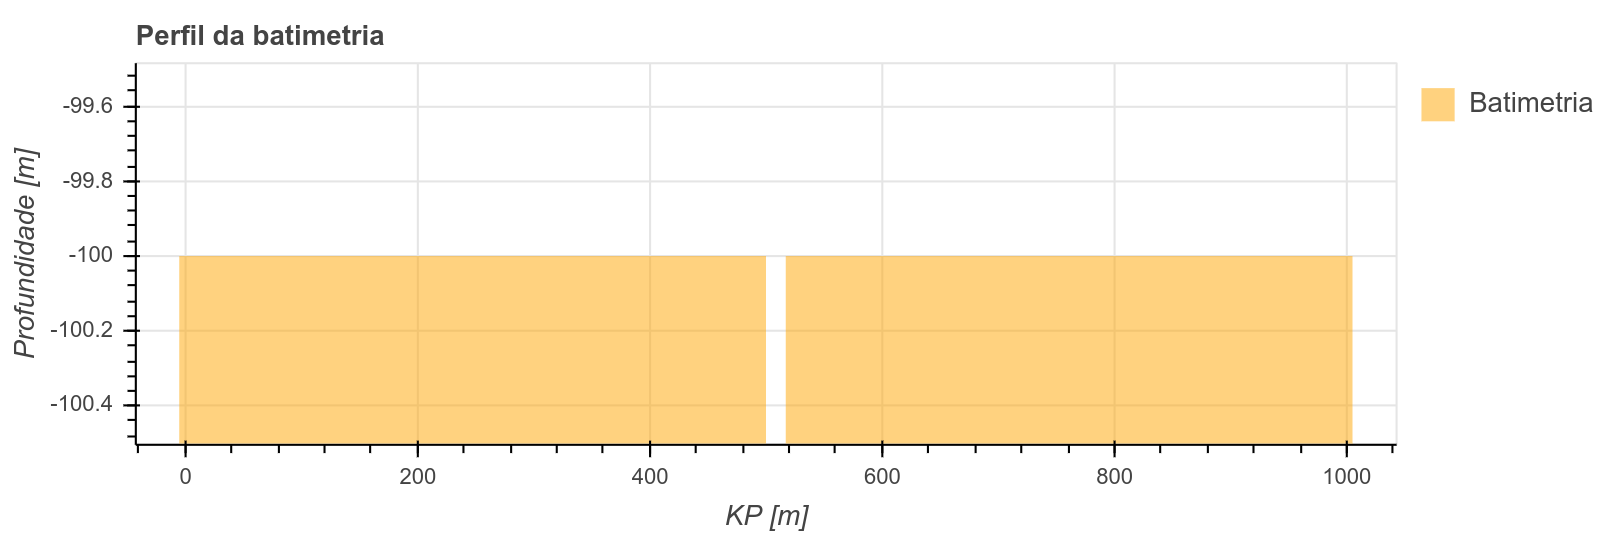
\includegraphics[width=\textwidth]{imagens/exemplo/ex_perfil_da_batimetriat.png}
    \fonte{Autor (2020)}
\end{figure}

A simulação realizada tem a seguinte sequência de passos de carga:

\begin{enumerate}
	\item Aplica-se o peso do duto vazio;
	\item Aplica-se a pressão externa;
	\item Aplica-se a tração de lançamento;
	\item Aplica-se o deslocamento vertical e assenta-se o duto;
	\item Restaura-se o atrito axial;
	\item Ativa-se as molas;
	\item Remove-se a tração de lançamento;
	\item Aplica-se a pressão do teste hidrostático;
	\item Remove-se a pressão do teste hidrostático;
	\item Aplica-se a pressão operacional;
	\item Obtêm-se os modos de vibração (análise modal).
\end{enumerate}

% Os valores dos carregamentos estão presentes na \autoref{tab:carregamentos}.

% \begin{table}[h]
% 	\renewcommand{\arraystretch}{1.2}
% 	\small
% 	\centering
% 	\caption{\label{tab:carregamentos} Carregamentos do duto.}
% 	\begin{tabular}{lcr}
% 		\toprule
% 		Característica & Unidade & Valor\\
% 		\midrule
% 		Pressão externa & kgf/cm$^2$ & 160\\
% 		Coeficiente de atrito transversal & & 0,9\\
% 		Coeficiente de atrito longitudinal & & 0,6\\
% 		Tração Residual de Lançamento & kN & 60\\
% 		Pressão do teste hidrostático & kgf/cm$^2$ & 160\\
% 		Pressão operacional & kgf/cm$^2$ & 160\\
% 		\bottomrule
% 	\end{tabular}
% \end{table}

A geração dos arquivos para simulação no ABAQUS contendo as instruções para toda essa sequência de passo é realizada usando o método \texttt{write\_inps}: \texttt{model.write\_inps()}.
Isso deve gerar dois arquivos dentro de um diretório chamado \texttt{exemplo}: o arquivo principal \texttt{exemplo.inp}, e \texttt{bt\_exemplo.inp}, com as coordenadas que define o perfil de batimetria. \par

O método \texttt{run\_abaqus} do objeto \texttt{model} é responsável por executar a chamada do ABAQUS de maneira programática para iniciar a simulação.
Nesse método, ocorre a leitura do arquivo de registro da simulação e o seu conteúdo é exibido na tela do console a cada \unit[5]{s}.

Uma vez terminada a simulação, a extração de dados do arquivo \texttt{odb} gerado pelo ABAQUS e o respectivo pós-processamento podem ser realizados com a chamada do método \texttt{post\_processing} do objeto \texttt{model}.
Há uma função para representação gráfica de cada um dos principais tipos de dados extraídos. A seguir, serão apresentadas algumas dessas funções e as respectivas figuras geradas por eles.

Em geral, a primeira forma de validação é uma inspeção visual da configuração deformada do duto sobre a batimetria. Desta forma é possível ver se a simulação consegue reproduzir a situação \textit{in-loco}, especialmente os vãos. Uma vez que a etapa anterior tenha gerado os arquivos \texttt{deformed\_shape.csv} (com as coordenadas da configuração deformada do duto) e \texttt{seabed.csv}, (com as coordenadas da batimetria), pode-se gerar um gráfico com o perfil do duto. O código para geração do gráfico desejado é semelhante ao exposto na \autoref{code:deformada}, e o gráfico resultante na \autoref{fig:ex-config-deformada}. Este e outros gráficos mais comuns são gerados automaticamente com uma chamada do método \texttt{make\_plots} do objeto \texttt{model}: \texttt{model.make\_plots()}.

\begin{figure}[!ht]
\caption{Código para geração do gráfico do perfil da configuração deformada do duto sobre a batimetria.}\label{code:deformada}
\begin{pythoncode}
deformed_shape = load_csv(model.final_results_folder / "deformed_shape.csv")
pipe_plot = plots.pipe_profile(deformed_shape, legend="Eixo do duto")
seabed = load_csv(model.final_results_folder / "seabed.csv")
pipe_plot.title = "Configuração deformada"
seabed_plot = plots.bathymetry(seabed)
seabed_pipe_plot = pipe_plot + seabed_plot
seabed_pipe_plot.set_range(y=(-0.06, 0.06), x=(400, 600))
seabed_pipe_plot.save("configuração_deformada.html")
\end{pythoncode}
\fonte{Autor (2020)}
\end{figure}

Vale destacar o uso do operador de adição (\texttt{+}) na linha 6. Com ele, é possível combinar dois gráficos (instâncias da classe Plot), sobrepondo-os em um mesmo gráficos.

\begin{figure}[!ht]
	\centering
	\caption{Configuração deformada do duto após a simulação.}\label{fig:ex-config-deformada}
	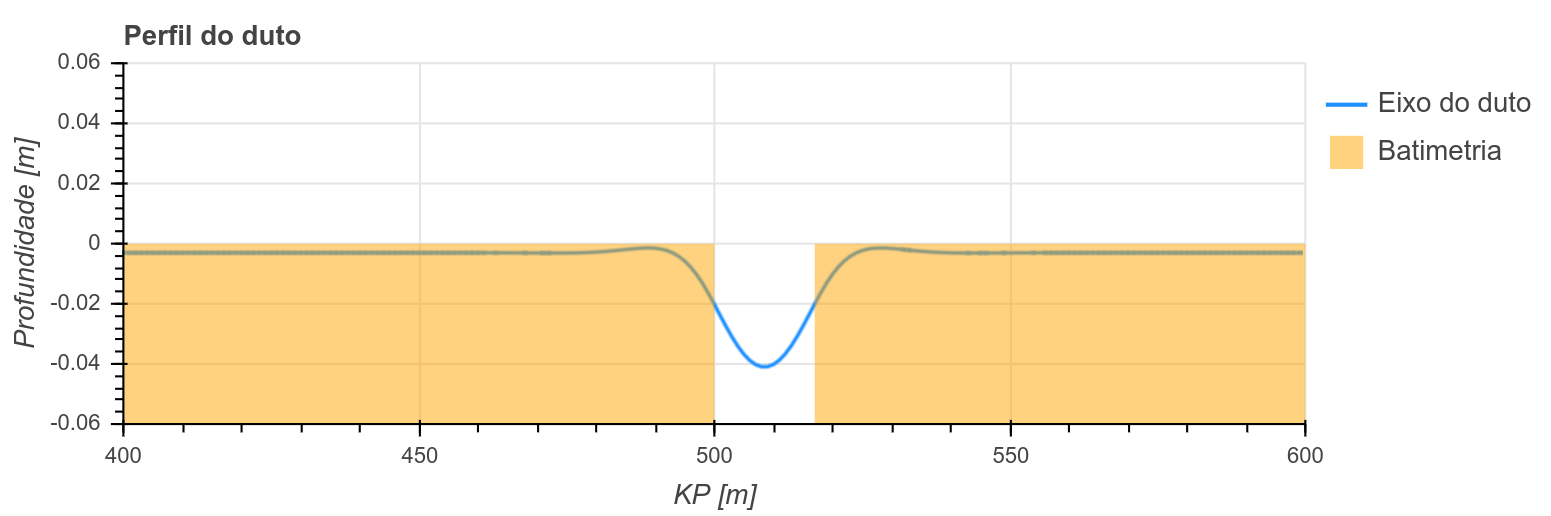
\includegraphics[width=\textwidth]{imagens/exemplo/deformada}
	\fonte{Autor (2020)}
\end{figure}

O próximo passo é a visualização dos modos de vibração com o objetivo de selecionar os que irão ser utilizados para o cálculo de fadiga. As Figuras~\ref{fig:all-modos-IL} e~\ref{fig:all-modos-CF} apresentam todos os modos de vibração computados pela análise modal do ABAQUS, separando-os em \textit{in-line} e \textit{cross-flow}, onde a região que compreende a extensão do vão está destacada com o fundo cinza.

\begin{figure}[H]
	\centering
	\caption{Modos de vibração \textit{in-line} geradas na análise modal.}\label{fig:all-modos-IL}
	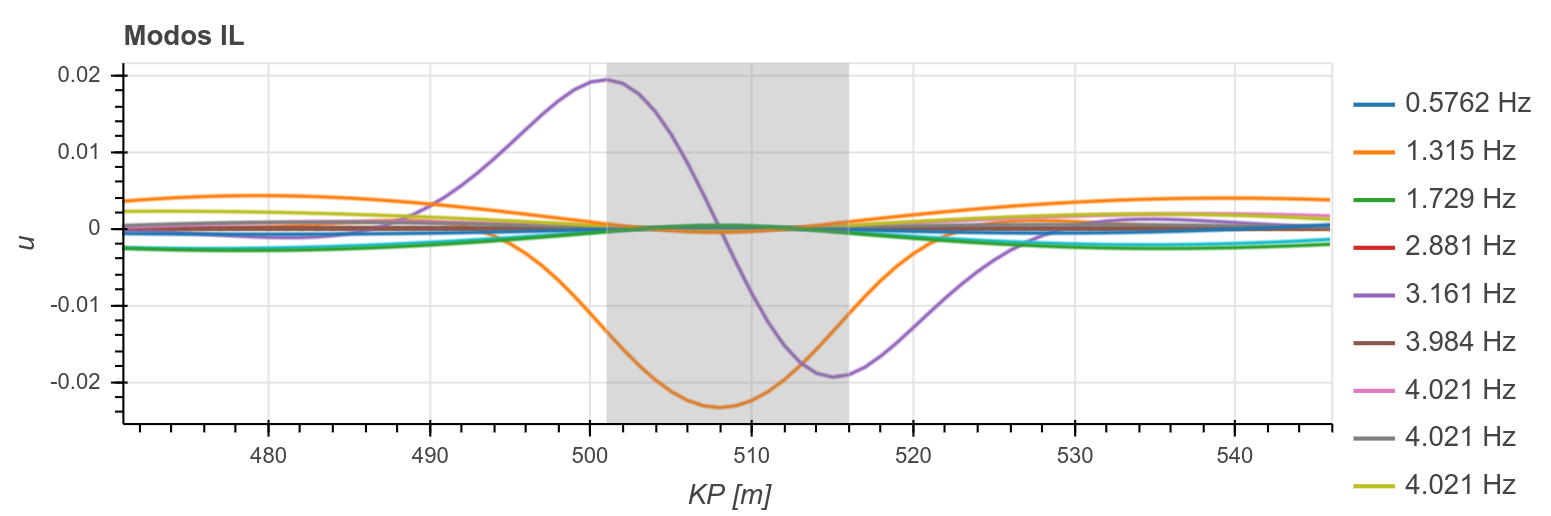
\includegraphics[width=\textwidth]{imagens/exemplo/all_modos_IL}
	\fonte{Autor (2020)}
\end{figure}

\begin{figure}[H]
	\centering
	\caption{Modos de vibração \textit{cross-flow} geradas na análise modal.}\label{fig:all-modos-CF}
	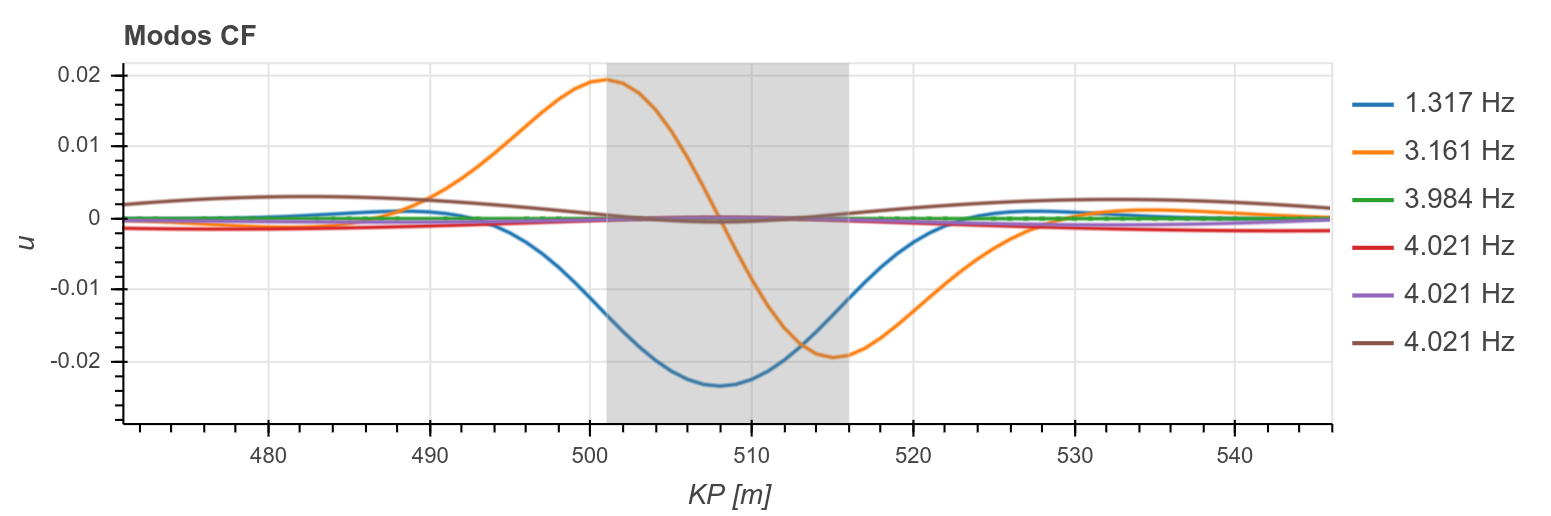
\includegraphics[width=\textwidth]{imagens/exemplo/all_modos_CF}
	\fonte{Autor (2020)}
\end{figure}

Como é possível ver nas Figuras~\ref{fig:all-modos-IL} e~\ref{fig:all-modos-CF}, há muitos modos espúrios, os quais devem ser desconsiderados da análise de fadiga. Esse é o papel do método \texttt{select\_modes} da classe \texttt{Span}. Esse método consiste na implementação dos processos de seleção de modos recomendados pela \dnvf105, apresentados na~\autoref{sec:multimode}. Para o exemplo aqui ilustrado, os resultados são os modos exibidos nas Figuras~\ref{fig:modos-IL} e~\ref{fig:modos-CF}.

\begin{figure}[!ht]
	\centering
	\caption{Modos de vibração \textit{in-line} selecionados pelo algoritmo implementado.}\label{fig:modos-IL}
	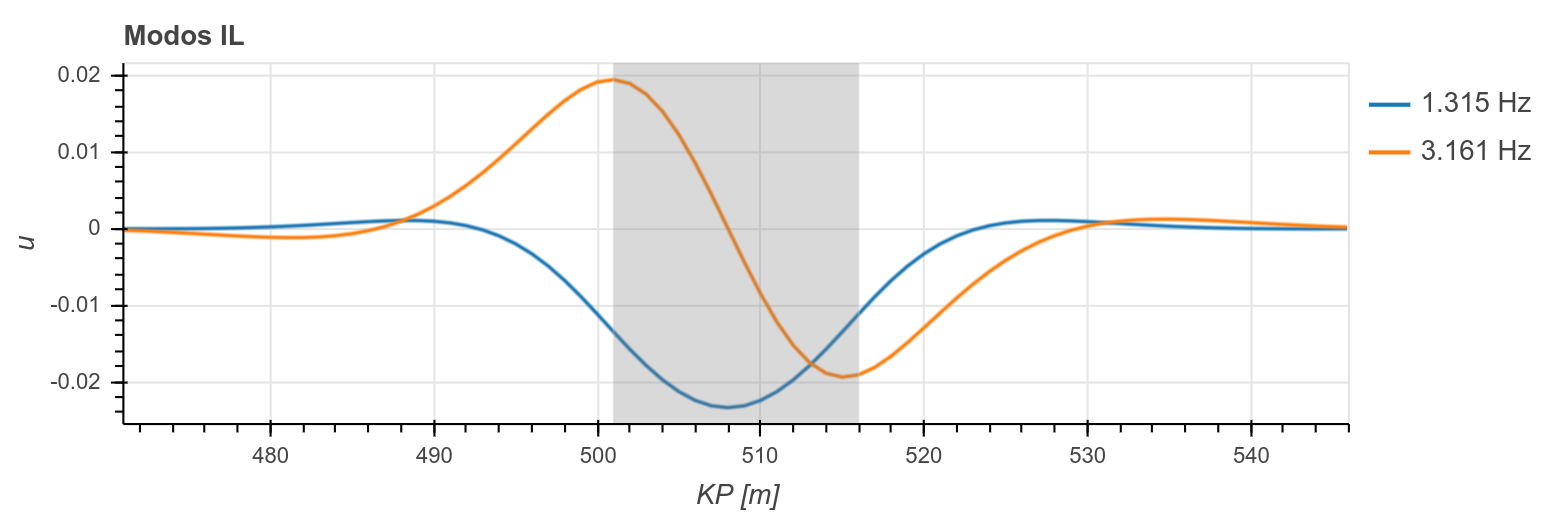
\includegraphics[width=\textwidth]{imagens/exemplo/modos_IL}
	\fonte{Autor (2020)}
\end{figure}

\begin{figure}[!ht]
	\centering
	\caption{Modos de vibração \textit{cross-flow} selecionados pelo algoritmo implementado.}\label{fig:modos-CF}
	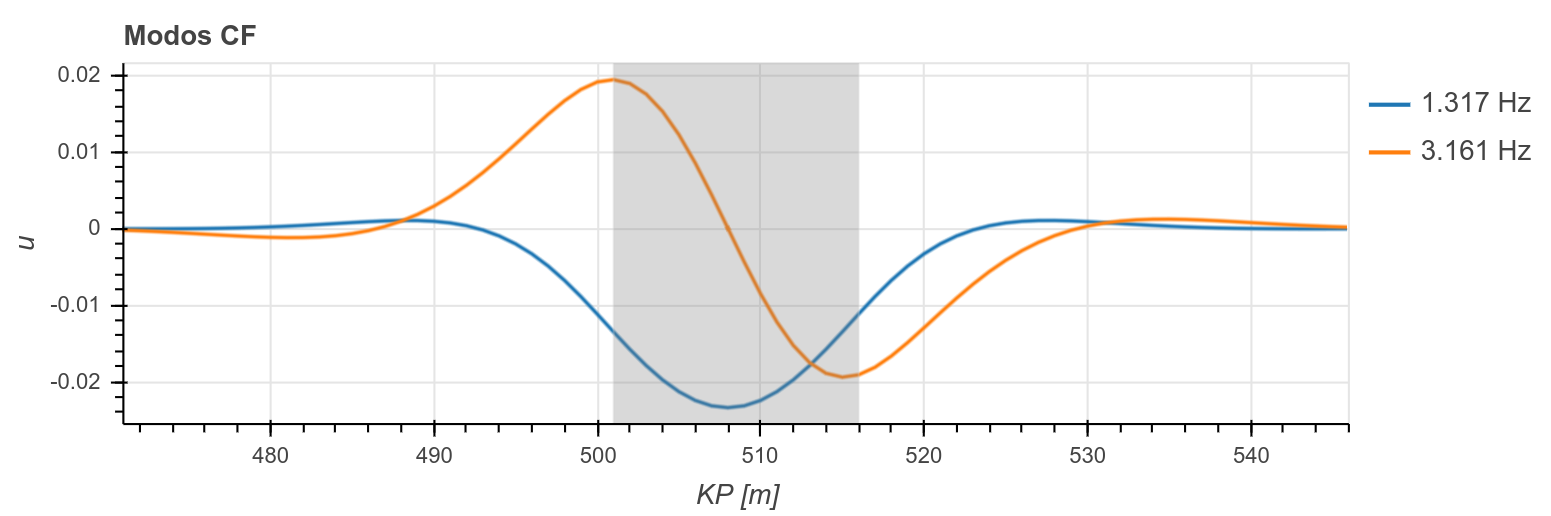
\includegraphics[width=\textwidth]{imagens/exemplo/modos_CF}
	\fonte{Autor (2020)}
\end{figure}

Estando satisfeito com os modos selecionados na etapa anterior, o usuário pode usar o método \texttt{run\_fatfree}, para que seja feita o preenchimento de uma instância da planilha com os dados específicos do vão, modos, e dados mais gerais, como condições ambientais e coeficientes de segurança. Um exemplo da massiva entrada de dados necessária nesse processo acontece na aba \textit{Multimode} da \fatfree, onde se faz a entrada das coordenadas dos modos de vibração (colunas em azul), conforme é possível ver na \autoref{fig:fatfree-multimode}.

\begin{figure}[!ht]
	\centering
	\caption{Dados inseridos na aba \textit{Multimode} da FatFree.}\label{fig:fatfree-multimode}
	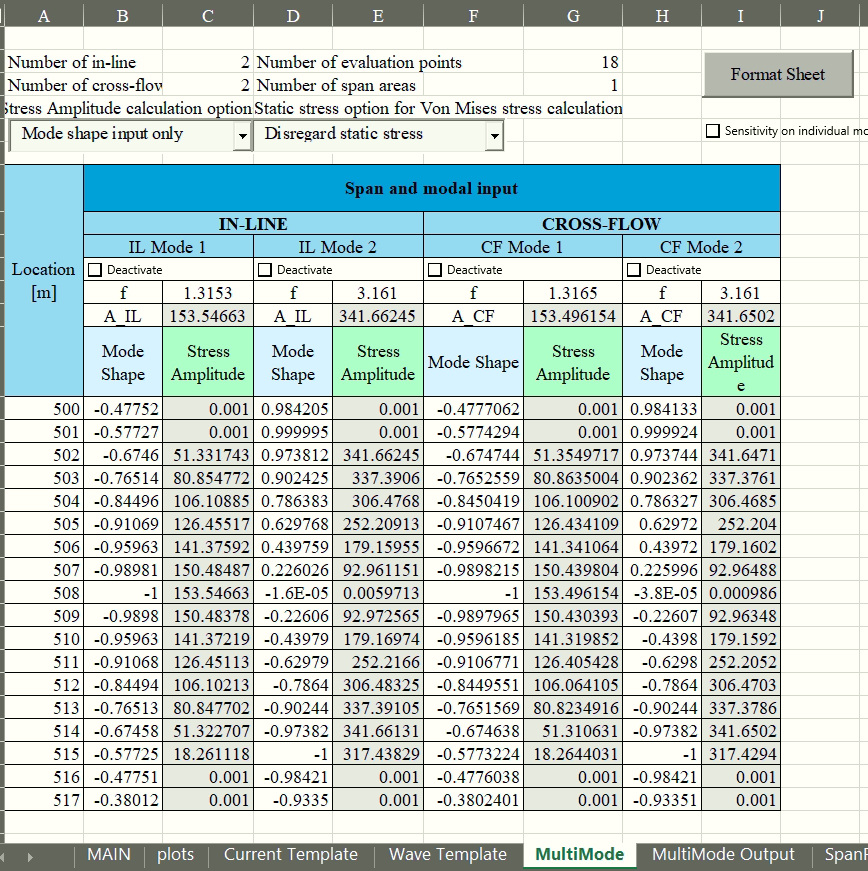
\includegraphics[width=0.6\textwidth]{imagens/exemplo/fatfree_multimode}
	\fonte{Autor {2020}}
\end{figure}

Com essa instância da planilha, tem-se outro ponto para validação dos resultados.
Segundo o item 6.7.4 da \dnvf105, a análise de elementos finitos para um único vão com $L / D_s \approx 60$, as frequências naturais de \textit{in-line} e \textit{cross-flow} e as faixas de tensão devem mostrar valores semelhantes com margem de $\pm$5\%, considerando esforço axial efetivo nulo ($S_{eff} = 0$). Para o modelo em questão, a comparação entre os valores da primeira frequência obtidos pela análise modal do ABAQUS e a \fatfree\ é apresentada na \autoref{tab:comparacao-frequencias}.

\begin{table}[!ht]
\renewcommand{\arraystretch}{1.2}
\centering
\caption{Comparação entre valores para a primeira frequência.}\label{tab:comparacao-frequencias}
\begin{tabular}{lrrr}
\toprule
Direção & ABAQUS & FatFree & Diferença relativa\\
\midrule
\textit{In-line}    & 1,315 & 1,351 & -2,66\%\\ % chktex 21
\textit{Cross-flow} & 1,317 & 1,357 & -2,95\%\\ % chktex 21
\bottomrule
\end{tabular}
\end{table}

Uma vez que se tenha atingido sucesso na tarefa de modelar o problema de modo a condizentes, pode-se agora usar a classe \texttt{FatFreeResults} para extrair os resultados de uma dada instância da \fatfree. Por exemplo, pode-se construir um gráfico da vida à fadiga ao longo do vão com perfil do duto com a batimetria abaixo dele (ver \autoref{fig:ex-config-deformada}), como mostra a \autoref{code:vida-a-fadiga}.

\begin{figure}[!ht]
	\caption{Código paa geração do gráficos de vida à fadiga.}\label{code:vida-a-fadiga}
	\begin{pythoncode}
from integrispan.dnv.fatfree_results import FatFreeResults
fatfree_results = FatFreeResults("FatFree_kp_508.5.xls", "./")
fatigue_life_plot = fatfree_results.plot_fatigue_life(baseline=20)
dashboard = fatigue_life_plot / seabed_pipe_plot
dashboard.save("fatigue_pipe_dashboard.html")
	\end{pythoncode}
	\fonte{Autor (2020)}
\end{figure}

Vale destacar o uso do operador de divisão (\texttt{/}) na linha 4. Com ele, é possível combinar dois gráficos (instâncias da classe Plot) posicionado-os um sobre o outro em um mesmo gráfico. O gráfico resultante é exibido na \autoref{fig:vida-a-fadiga}, onde se tem a vida à fadiga nas direções \textit{in-line} (IL Comb) e \textit{cross-flow} (CF RM) na região do vão, bem como uma linha de referência que ajuda a identificar os trechos cuja previsão de vida à fadiga está abaixo do esperado.

\begin{figure}[!ht]
	\centering
	\caption{Gráfico de vida à fadiga e perfil do duto.}\label{fig:vida-a-fadiga}
	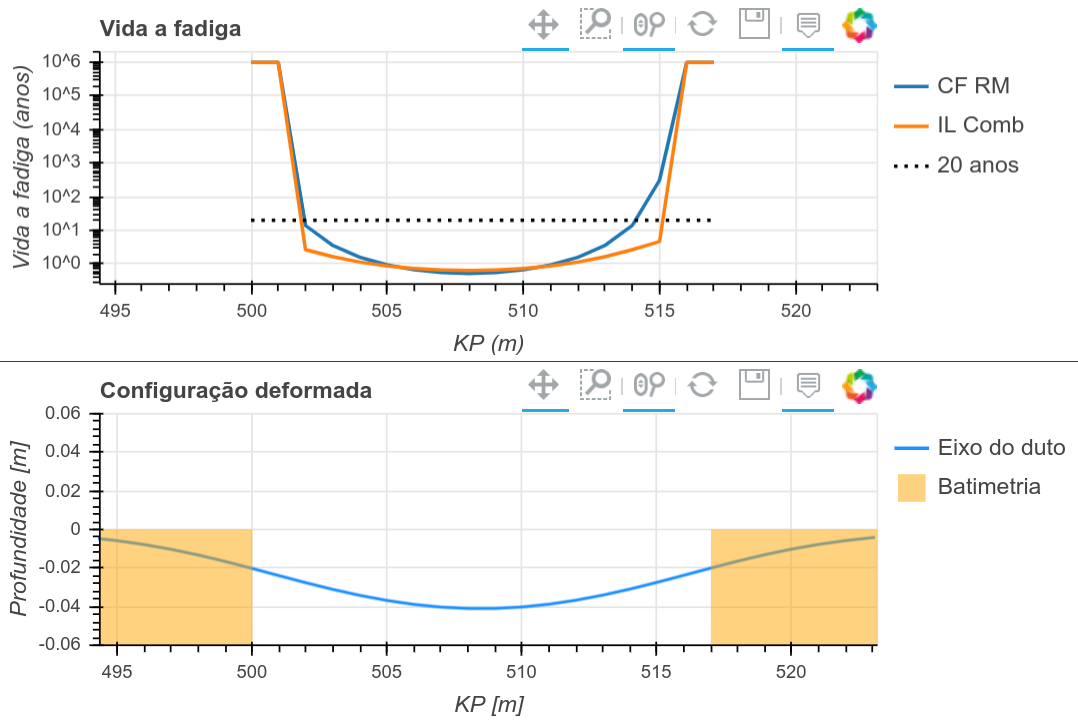
\includegraphics[width=\textwidth]{imagens/exemplo/vida-a-fadiga}
	\fonte{Autor (2020)}
\end{figure}

Por fim, vale destacar que a execução dos códigos pertencentes a ferramenta apresentadas neste capítulos levam não mais que poucos segundos cada. Isso representa uma redução de tempo significativa em relação ao cenário sem uso da ferramenta, onde esses processo poderia levar de horas a dias. Os ganho se concentram principalmente nas operações em que envolvem a maior quantidade de dados como a geração do representação da batimetria na modelagem de elementos finitos e no preenchimento da \fatfree\ com os dados nos modos de vibração.